% Options for packages loaded elsewhere
\PassOptionsToPackage{unicode}{hyperref}
\PassOptionsToPackage{hyphens}{url}
\PassOptionsToPackage{dvipsnames,svgnames,x11names}{xcolor}
%
\documentclass[
  letterpaper,
  DIV=11,
  numbers=noendperiod,
  oneside]{scrartcl}

\usepackage{amsmath,amssymb}
\usepackage{iftex}
\ifPDFTeX
  \usepackage[T1]{fontenc}
  \usepackage[utf8]{inputenc}
  \usepackage{textcomp} % provide euro and other symbols
\else % if luatex or xetex
  \usepackage{unicode-math}
  \defaultfontfeatures{Scale=MatchLowercase}
  \defaultfontfeatures[\rmfamily]{Ligatures=TeX,Scale=1}
\fi
\usepackage{lmodern}
\ifPDFTeX\else  
    % xetex/luatex font selection
\fi
% Use upquote if available, for straight quotes in verbatim environments
\IfFileExists{upquote.sty}{\usepackage{upquote}}{}
\IfFileExists{microtype.sty}{% use microtype if available
  \usepackage[]{microtype}
  \UseMicrotypeSet[protrusion]{basicmath} % disable protrusion for tt fonts
}{}
\makeatletter
\@ifundefined{KOMAClassName}{% if non-KOMA class
  \IfFileExists{parskip.sty}{%
    \usepackage{parskip}
  }{% else
    \setlength{\parindent}{0pt}
    \setlength{\parskip}{6pt plus 2pt minus 1pt}}
}{% if KOMA class
  \KOMAoptions{parskip=half}}
\makeatother
\usepackage{xcolor}
\usepackage[left=1in,marginparwidth=2.0666666666667in,textwidth=4.1333333333333in,marginparsep=0.3in]{geometry}
\setlength{\emergencystretch}{3em} % prevent overfull lines
\setcounter{secnumdepth}{-\maxdimen} % remove section numbering
% Make \paragraph and \subparagraph free-standing
\ifx\paragraph\undefined\else
  \let\oldparagraph\paragraph
  \renewcommand{\paragraph}[1]{\oldparagraph{#1}\mbox{}}
\fi
\ifx\subparagraph\undefined\else
  \let\oldsubparagraph\subparagraph
  \renewcommand{\subparagraph}[1]{\oldsubparagraph{#1}\mbox{}}
\fi


\providecommand{\tightlist}{%
  \setlength{\itemsep}{0pt}\setlength{\parskip}{0pt}}\usepackage{longtable,booktabs,array}
\usepackage{calc} % for calculating minipage widths
% Correct order of tables after \paragraph or \subparagraph
\usepackage{etoolbox}
\makeatletter
\patchcmd\longtable{\par}{\if@noskipsec\mbox{}\fi\par}{}{}
\makeatother
% Allow footnotes in longtable head/foot
\IfFileExists{footnotehyper.sty}{\usepackage{footnotehyper}}{\usepackage{footnote}}
\makesavenoteenv{longtable}
\usepackage{graphicx}
\makeatletter
\def\maxwidth{\ifdim\Gin@nat@width>\linewidth\linewidth\else\Gin@nat@width\fi}
\def\maxheight{\ifdim\Gin@nat@height>\textheight\textheight\else\Gin@nat@height\fi}
\makeatother
% Scale images if necessary, so that they will not overflow the page
% margins by default, and it is still possible to overwrite the defaults
% using explicit options in \includegraphics[width, height, ...]{}
\setkeys{Gin}{width=\maxwidth,height=\maxheight,keepaspectratio}
% Set default figure placement to htbp
\makeatletter
\def\fps@figure{htbp}
\makeatother

\KOMAoption{captions}{tableheading}
\makeatletter
\@ifpackageloaded{tcolorbox}{}{\usepackage[skins,breakable]{tcolorbox}}
\@ifpackageloaded{fontawesome5}{}{\usepackage{fontawesome5}}
\definecolor{quarto-callout-color}{HTML}{909090}
\definecolor{quarto-callout-note-color}{HTML}{0758E5}
\definecolor{quarto-callout-important-color}{HTML}{CC1914}
\definecolor{quarto-callout-warning-color}{HTML}{EB9113}
\definecolor{quarto-callout-tip-color}{HTML}{00A047}
\definecolor{quarto-callout-caution-color}{HTML}{FC5300}
\definecolor{quarto-callout-color-frame}{HTML}{acacac}
\definecolor{quarto-callout-note-color-frame}{HTML}{4582ec}
\definecolor{quarto-callout-important-color-frame}{HTML}{d9534f}
\definecolor{quarto-callout-warning-color-frame}{HTML}{f0ad4e}
\definecolor{quarto-callout-tip-color-frame}{HTML}{02b875}
\definecolor{quarto-callout-caution-color-frame}{HTML}{fd7e14}
\makeatother
\makeatletter
\makeatother
\makeatletter
\makeatother
\makeatletter
\@ifpackageloaded{caption}{}{\usepackage{caption}}
\AtBeginDocument{%
\ifdefined\contentsname
  \renewcommand*\contentsname{Table of contents}
\else
  \newcommand\contentsname{Table of contents}
\fi
\ifdefined\listfigurename
  \renewcommand*\listfigurename{List of Figures}
\else
  \newcommand\listfigurename{List of Figures}
\fi
\ifdefined\listtablename
  \renewcommand*\listtablename{List of Tables}
\else
  \newcommand\listtablename{List of Tables}
\fi
\ifdefined\figurename
  \renewcommand*\figurename{Figure}
\else
  \newcommand\figurename{Figure}
\fi
\ifdefined\tablename
  \renewcommand*\tablename{Table}
\else
  \newcommand\tablename{Table}
\fi
}
\@ifpackageloaded{float}{}{\usepackage{float}}
\floatstyle{ruled}
\@ifundefined{c@chapter}{\newfloat{codelisting}{h}{lop}}{\newfloat{codelisting}{h}{lop}[chapter]}
\floatname{codelisting}{Listing}
\newcommand*\listoflistings{\listof{codelisting}{List of Listings}}
\makeatother
\makeatletter
\@ifpackageloaded{caption}{}{\usepackage{caption}}
\@ifpackageloaded{subcaption}{}{\usepackage{subcaption}}
\makeatother
\makeatletter
\@ifpackageloaded{tcolorbox}{}{\usepackage[skins,breakable]{tcolorbox}}
\makeatother
\makeatletter
\@ifundefined{shadecolor}{\definecolor{shadecolor}{rgb}{.97, .97, .97}}
\makeatother
\makeatletter
\makeatother
\makeatletter
\@ifpackageloaded{sidenotes}{}{\usepackage{sidenotes}}
\@ifpackageloaded{marginnote}{}{\usepackage{marginnote}}
\makeatother
\makeatletter
\makeatother
\ifLuaTeX
  \usepackage{selnolig}  % disable illegal ligatures
\fi
\IfFileExists{bookmark.sty}{\usepackage{bookmark}}{\usepackage{hyperref}}
\IfFileExists{xurl.sty}{\usepackage{xurl}}{} % add URL line breaks if available
\urlstyle{same} % disable monospaced font for URLs
\hypersetup{
  pdftitle={Lab 3: Peripheral Circulation and The Dive Response},
  pdfauthor={Marguerite Butler},
  colorlinks=true,
  linkcolor={blue},
  filecolor={Maroon},
  citecolor={Blue},
  urlcolor={Blue},
  pdfcreator={LaTeX via pandoc}}

\title{Lab 3: Peripheral Circulation and The Dive Response}
\author{Marguerite Butler}
\date{2023-09-01}

\begin{document}
\maketitle
\ifdefined\Shaded\renewenvironment{Shaded}{\begin{tcolorbox}[boxrule=0pt, breakable, borderline west={3pt}{0pt}{shadecolor}, interior hidden, enhanced, sharp corners, frame hidden]}{\end{tcolorbox}}\fi

\renewcommand*\contentsname{Table of contents}
{
\hypersetup{linkcolor=}
\setcounter{tocdepth}{3}
\tableofcontents
}
\hypertarget{before-lab}{%
\section{Before Lab}\label{before-lab}}

\begin{tcolorbox}[enhanced jigsaw, opacityback=0, colbacktitle=quarto-callout-note-color!10!white, opacitybacktitle=0.6, colback=white, leftrule=.75mm, title=\textcolor{quarto-callout-note-color}{\faInfo}\hspace{0.5em}{Prepare for lab by:}, breakable, rightrule=.15mm, colframe=quarto-callout-note-color-frame, bottomrule=.15mm, bottomtitle=1mm, arc=.35mm, toptitle=1mm, titlerule=0mm, toprule=.15mm, left=2mm, coltitle=black]

\begin{itemize}
\tightlist
\item
  Watch Peripheral Circulation Podcast.
\item
  Read {[}\href{../Protocols/p2-measuring-blood-pressure.pdf}{Protocol
  2}{]} on measuring blood pressure.
\item
  Read the lab manual below.\\
\item
  Write the
  {[}\href{../../labs-misc/lab-notebook.qmd\#sec-prelab}{Prelab}{]} in
  your lab notebook.
\item
  Do Quiz on Laulima (open 24 hrs before lab).
\end{itemize}

\url{https://youtu.be/h47oQH-w6F8}

\end{tcolorbox}

\begin{tcolorbox}[enhanced jigsaw, opacityback=0, colbacktitle=quarto-callout-note-color!10!white, opacitybacktitle=0.6, colback=white, leftrule=.75mm, title=\textcolor{quarto-callout-note-color}{\faInfo}\hspace{0.5em}{Exercises}, breakable, rightrule=.15mm, colframe=quarto-callout-note-color-frame, bottomrule=.15mm, bottomtitle=1mm, arc=.35mm, toptitle=1mm, titlerule=0mm, toprule=.15mm, left=2mm, coltitle=black]

\begin{itemize}
\tightlist
\item
  Measuring blood pressure
\item
  Peripheral circulation experiment

  \begin{itemize}
  \tightlist
  \item
    Develop a simple experiment to demonstrate a principle of peripheral
    circulation of choice.
  \end{itemize}
\item
  Dive response experiment

  \begin{itemize}
  \tightlist
  \item
    Develop a hypothesis for a potential trigger for the dive response.
  \end{itemize}
\end{itemize}

\end{tcolorbox}

\hypertarget{background-blood-pressure-and-peripheral-circulation}{%
\section{Background: Blood pressure and peripheral
circulation}\label{background-blood-pressure-and-peripheral-circulation}}

Vertebrates have a \textbf{closed circulatory system} where the blood is
always enclosed within blood vessels or the heart. Blood is pumped from
the \textbf{heart} (the central pump) to the \textbf{vasculature}: the
\textbf{arteries}, \textbf{capillary beds} (sites of delivery to
tissues), \textbf{the veins}, and back to heart. There are several
important consequences of this design: (1) blood pressure varies across
species according to oxygen demand and morphology (especially animal
height), (2) \textbf{blood pressure varies along the circuit}, (3)
\textbf{blood pressure can be regulated at points along the circuit},
and (4) \textbf{blood pressure can be modified situationally} depending
the state of the animal.

\hypertarget{blood-pressure-varies-across-species}{%
\subsubsection{Blood pressure varies across
species}\label{blood-pressure-varies-across-species}}

For \textbf{very active} animals (e.g., mammals and birds) or
\textbf{very large animals} (especially very tall animals that have more
gravity to resist), the ability to regulate blood pressure is critical
--- active animals will \emph{need more oxygen delivered at a faster
rate}, especially to the most metabolically active tissues, and
\emph{larger animals will require much more pressure} to reach all of
their tissues.

\hypertarget{blood-pressure-varies-during-the-cardiac-cycle.}{%
\subsubsection{Blood pressure varies during the cardiac
cycle.}\label{blood-pressure-varies-during-the-cardiac-cycle.}}

The \textbf{cardiac cycle} is a complete cycle of the heart beat,
comprised of \textbf{systole} (Figure~\ref{fig-systole}; the phase
involving contraction and ejection) and \textbf{diastole}
(Figure~\ref{fig-diastole}; relaxation and filling) of the atria and
ventricles. We will learn more about the cardiac cycle in the EKG lab.
In this lab we are focusing on the blood pressure changes. The largest
muscles of the heart are in the \textbf{ventricles}. Blood pressure is
at its highest immediately after the ventricles contract to push blood
into the arterial system (Figure~\ref{fig-wiggers}; \textbf{systolic
pressure}) and declines as the ventricles relax to fill with blood
before pumping again. Just before the ventricles contract, blood
pressure is at its lowest (\textbf{diastolic pressure}).

\begin{marginfigure}

{\centering 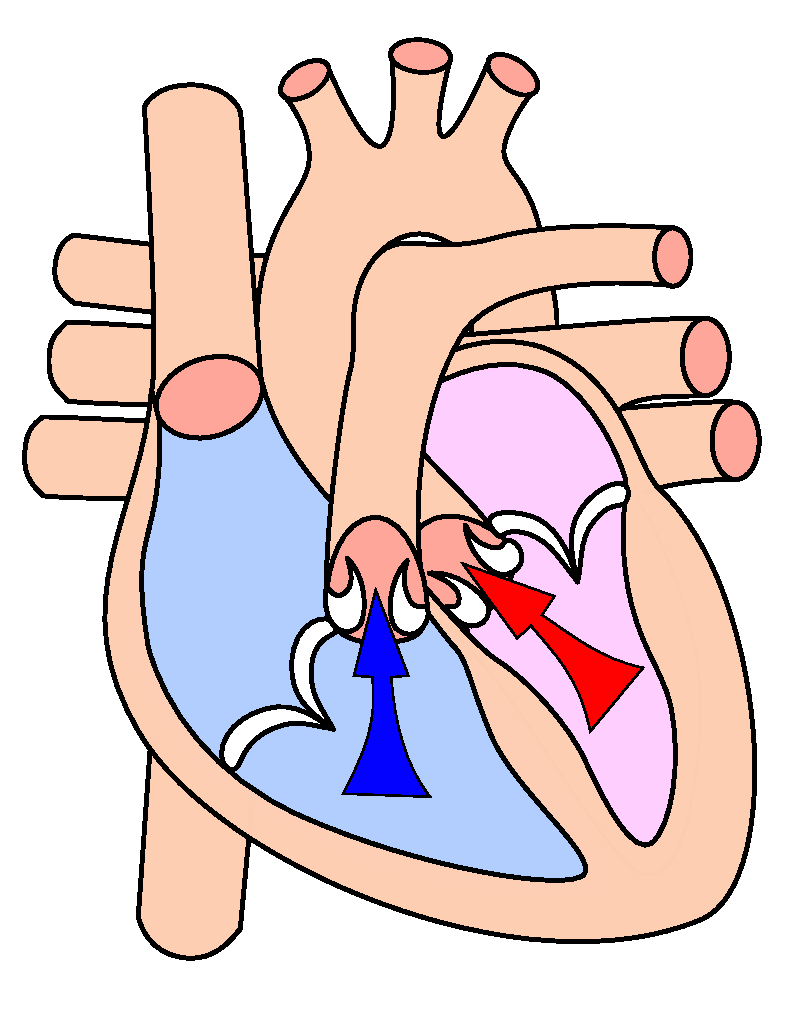
\includegraphics{Lab3_files/mediabag/../../images/Heart_systole.pdf}

}

\caption{\label{fig-systole}The human heart during the ventricular
\textbf{systole} phase of the \textbf{cardiac cycle}. Image by
\href{https://en.wikipedia.org/wiki/User:Wapcaplet}{Wapcaplet},
\href{https://commons.wikimedia.org/wiki/User:Reytan}{Reytan},
\href{https://commons.wikimedia.org/wiki/User:Mtcv}{Mtcv} /
\href{https://commons.wikimedia.org/wiki/File:Heart_systole.svg}{Heart
systole}/\href{https://creativecommons.org/licenses/by-sa/3.0/}{CC BY-SA
3.0}}

\end{marginfigure}

\begin{marginfigure}

{\centering 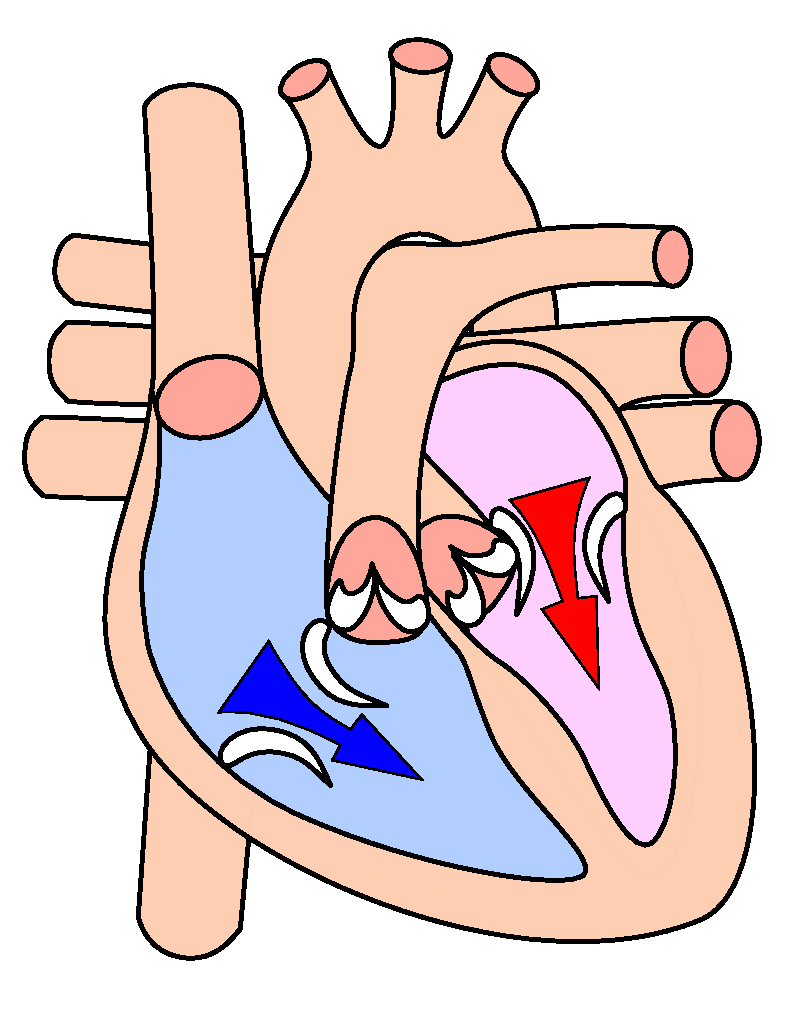
\includegraphics{Lab3_files/mediabag/../../images/Heart_diasystole.pdf}

}

\caption{\label{fig-diastole}The heart relaxes and the ventricles fill
during the \textbf{diastole} phase of the \textbf{cardiac cycle}. Image
by \href{https://en.wikipedia.org/wiki/User:Wapcaplet}{Wapcaplet},
\href{https://commons.wikimedia.org/wiki/User:Reytan}{Reytan},
Vector:\href{https://commons.wikimedia.org/wiki/User:Sjef}{Sjef} /
\href{https://commons.wikimedia.org/wiki/File:Heart_diasystole.svg}{Heart
diastole}/ \href{https://creativecommons.org/licenses/by-sa/3.0/}{CC
BY-SA 3.0}}

\end{marginfigure}

\begin{figure}

{\centering 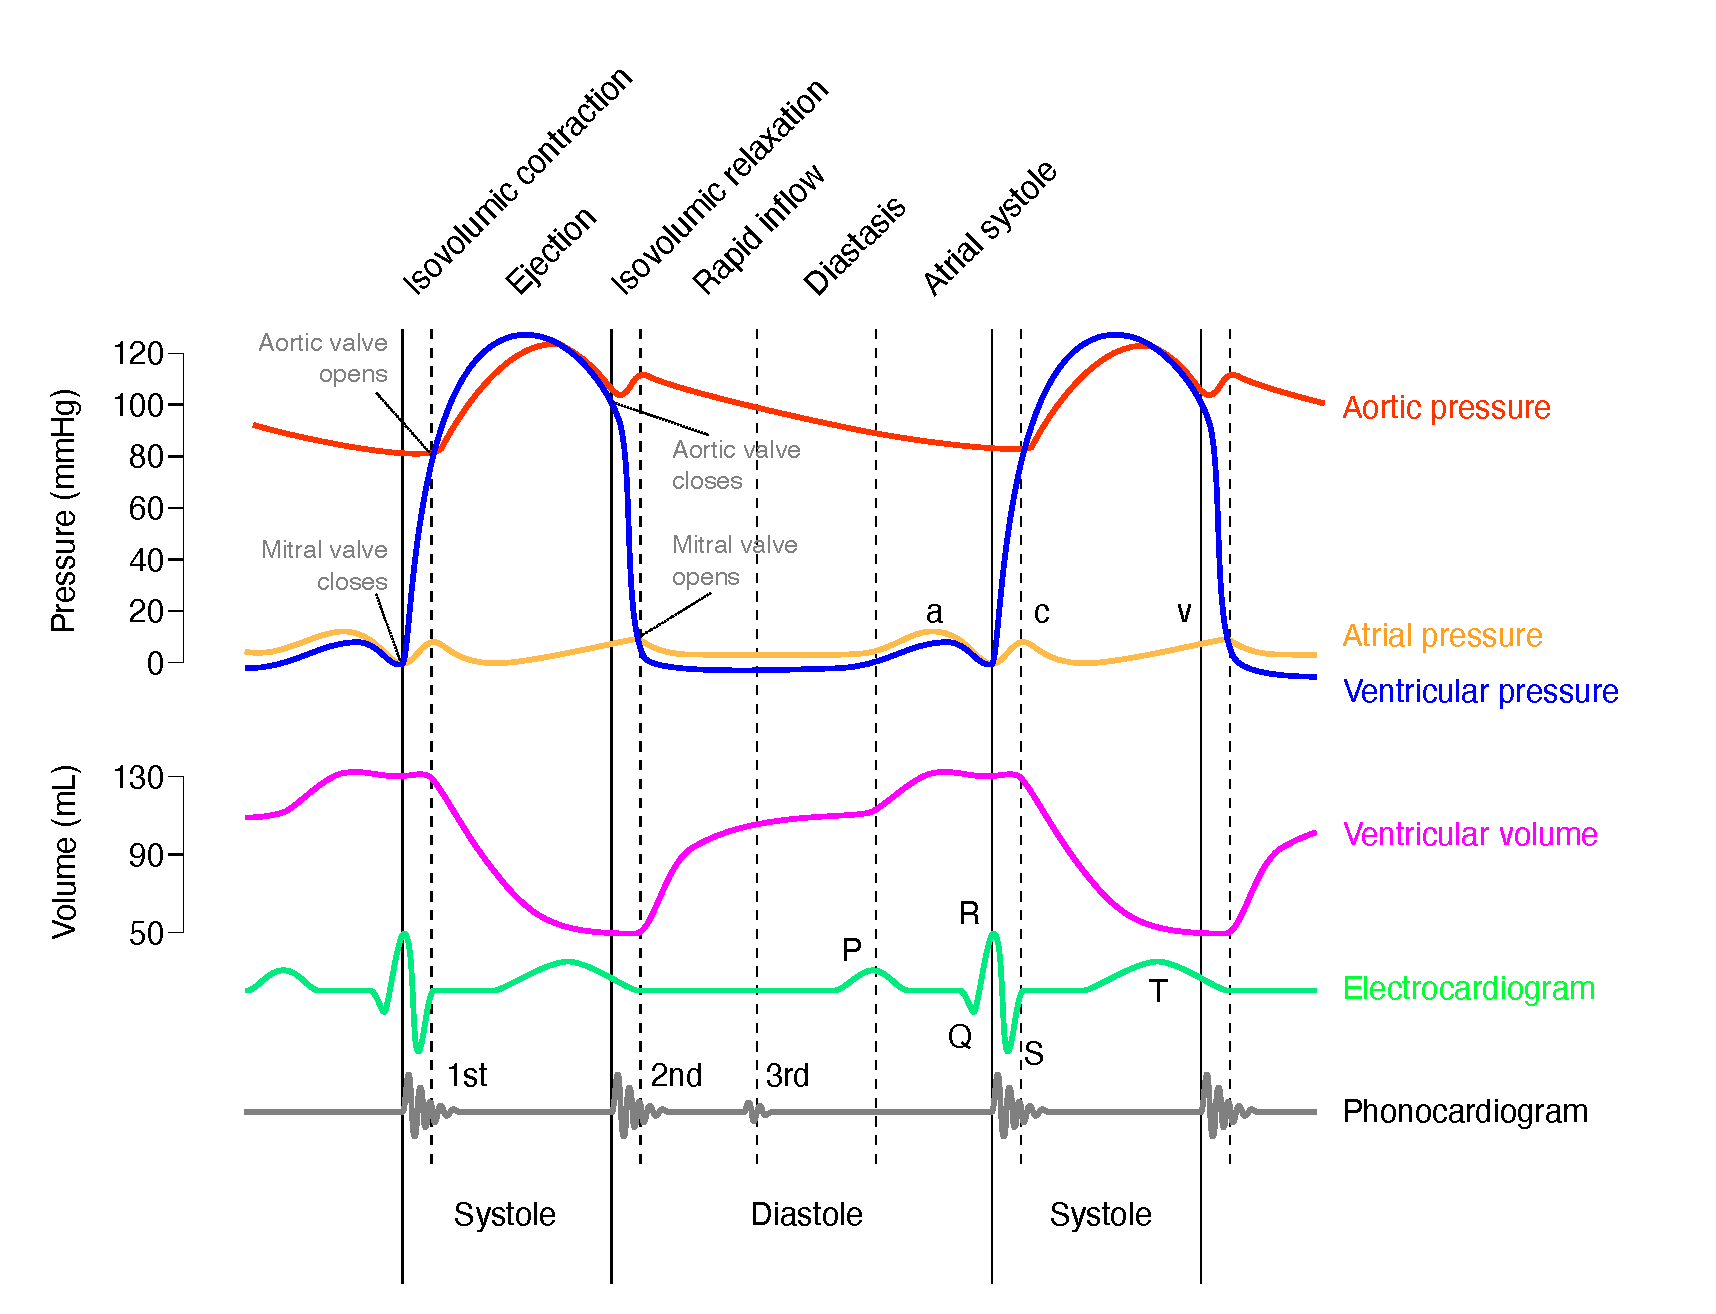
\includegraphics{Lab3_files/mediabag/../../images/Wiggers_Diagram_2.pdf}

}

\caption{\label{fig-wiggers}Volume and pressure changes during the
\textbf{cardiac cycle}, as shown in a Wiggers diagram. Note that aortic
and ventricular pressures are both lowest and the end of diastole, just
before the beginning of systole. adh30 revised work by DanielChangMD who
revised original work of DestinyQx; Redrawn as SVG by xavax,
\href{https://commons.wikimedia.org/wiki/File:Wiggers_Diagram_2.svg}{Wiggers
Diagram 2},
\href{https://creativecommons.org/licenses/by-sa/4.0/legalcode}{CC BY-SA
4.0}}

\end{figure}

\hypertarget{blood-pressure-varies-along-the-vascular-circuit.}{%
\subsubsection{Blood pressure varies along the vascular
circuit.}\label{blood-pressure-varies-along-the-vascular-circuit.}}

Blood in the arteries leaving the heart is always at very high pressure
as compared to the low pressure in the veins in the legs or the even
lower pressure in capillary beds at the tissues. Blood pressure drops as
the blood vessels branch again and again, increasing the cross-sectional
area of the circuit, until it reaches the capillaries where the tissues
experience relatively constant, low pressure to facilitate
\textbf{diffusion}.

The slow blood flow at the capillaries facilitates diffusion of oxygen,
nutrients, and carbon dioxide and other wastes between the blood and the
tissues that are bathed by the capillaries. Therefore, \textbf{pressure
varies} depending on \textbf{distance from the heart}, the
\textbf{cross-sectional area of the blood vessels}, as well as
\textbf{gravity}. However, at any given point along the circuit, blood
pressure remains fairly constant.

\hypertarget{circulation-can-be-adjusted-situationally.}{%
\subsubsection{Circulation can be adjusted
situationally.}\label{circulation-can-be-adjusted-situationally.}}

At most times, blood pressure is regulated to \textbf{maintain a
relatively constant pressure}, however, there are times when
\textbf{circulation needs to be adjusted}. A well-known example is the
\textbf{Fight-or-Flight response}, which occurs, for example, when an
animal sees a predator or anticipates a fight. The \textbf{sympathetic
nervous system} dominates and causes a ramp-up of circulation to deliver
more energy to the skeletal muscles: increased \textbf{cardiac output}
(= \textbf{heart rate} x \textbf{stroke volume}) and \textbf{blood
pressure}, and increased blood flow to the lungs and skeletal muscles.
In contrast, the \textbf{rest-and-digest} response occurs after an
animal has had a large meal. The \textbf{parasympathetic nervous system}
dominates, lowering heart rate, concentrates blood flow to the gut, and
promotes a resting state.

Adjustments to blood flow are not simply an adjustment of heart
function, but also \textbf{constriction or relaxation of the
vasculature} (blood vessels: arteries, veins, capillaries).
\textbf{Constricting blood vessels} will reduce their
\textbf{cross-sectional area} and \textbf{increase blood pressure and
flow}.

Local changes in circulation are under \textbf{nervous} and
\textbf{hormonal} control. Regulation of blood flow in the vertebrate
circulatory system occurs by three primary mechanisms: 1) \textbf{local
receptors} (\emph{nervous system}) to detect levels of metabolic
activity (e.g., carbon dioxide receptors), 2) \textbf{sympathetic} and
\textbf{parasympathetic} (\emph{autonomic nervous system}) control of
the vasculature including capillary beds at the tissues, and 3)
\textbf{endocrine} (\emph{hormonal}) control of the vasculature.

In this lab, we will measure blood pressure of volunteers using a finger
pulse transducer, a stethoscope, a blood pressure cuff
(sphygnomanometer), and changes in peripheral circulation by measuring
the volume of the extremities using a belt with a force transducer. We
will do a series of learning exercises and then conduct an experiment on
factors affecting peripheral circulation and as well as during simulated
dives (the dive response).

\hypertarget{equipment}{%
\subsection{Equipment}\label{equipment}}

\begin{itemize}
\tightlist
\item
  PowerLab data acquisition system
\item
  Finger pulse transducer
\item
  Stethoscope
\item
  Blood pressure cuff
\item
  Blood pressure gauge (sphygnomanometer) with pod or BNC port
\item
  Respiratory belt transducer
\item
  LabChart software, note Blood Pressure settings
\end{itemize}

\hypertarget{exercise-1-measuring-blood-pressure}{%
\section{Exercise 1: Measuring Blood
Pressure}\label{exercise-1-measuring-blood-pressure}}

Traditionally, systemic arterial blood pressure is measured using a
\textbf{stethoscope} and a \textbf{blood pressure cuff} connected to a
blood pressure gauge called a \textbf{sphygnomanometer}
(\emph{sss-fig-no-ma-nom-eter}). The sphygnomanometer is calibrated in
pressure units of mmHg (millimeters of mercury). Modern instruments use
compressed air as a hydraulic fluid to transmit the force of your
pulsing blood.

Refer to {[}\href{../Protocols/p2-measuring-blood-pressure.pdf}{Protocol
2.1 and 2.2}{]} for how to measure blood pressure.

\hypertarget{setup}{%
\subsection{Setup}\label{setup}}

\begin{enumerate}
\def\labelenumi{\arabic{enumi}.}
\tightlist
\item
  Use ``Blood Pressure'' settings to start Chart software.
\item
  Setup Finger Pulse transducer on Input 1.
\item
  Attach sphygmomanometer transducer to Input 2 (pod input).
\end{enumerate}

\hypertarget{data-collection}{%
\subsection{Data Collection}\label{data-collection}}

\begin{enumerate}
\def\labelenumi{\arabic{enumi}.}
\tightlist
\item
  Measure blood pressure on a human volunteer using
  \textbf{auscultation} (listening through a stethoscope) and a
  \textbf{sphygnamonometer} .
\item
  Measure blood pressure using the PowerLab system and LabChart. Check
  that the \textbf{channel settings} are correctly set for each channel.
\item
  Repeat (1) and (2) on each group member, making sure to comment your
  data trace.
\end{enumerate}

\hypertarget{questions-for-thought}{%
\subsubsection{Questions for
thought\ldots{}}\label{questions-for-thought}}

\begin{enumerate}
\def\labelenumi{\arabic{enumi}.}
\tightlist
\item
  Does the time of the first \textbf{Korotkoff sound} (systolic pressure
  heard through the stethoscope), correspond with the first appearance
  of blood flow (as measured by the finger pulse)? Why or why not?
\item
  Would slowing the rate of pressure release from the cuff make your
  readings of the first appearance of blood flow more accurate? What
  problems might be caused by slowing pressure release?
\item
  Does the time that diastolic pressure is heard through the stethoscope
  correspond with anything particular in the blood flow signal? Can you,
  therefore, use pulse measurement to replace the stethoscope?
\item
  How much variation in measurement of diastolic and systolic pressures
  was observed within and between individuals? What are potential
  sources of variation in these estimates?
\end{enumerate}

\hypertarget{exercise-2-exploring-peripheral-circulation}{%
\section{Exercise 2: Exploring Peripheral
Circulation}\label{exercise-2-exploring-peripheral-circulation}}

\hypertarget{objectives}{%
\subsection{Objectives}\label{objectives}}

To demonstrate basic principles of peripheral circulation using blood
pressure data from the extremities. What you would expect based on
relative distance from the heart and gravity (and whether the location
is above or below the heart)?

\hypertarget{procedure}{%
\subsection{Procedure}\label{procedure}}

\begin{enumerate}
\def\labelenumi{\arabic{enumi}.}
\tightlist
\item
  \emph{Brainstorm with your lab group to develop some simple
  experiments to demonstrate principles of peripheral circulation.} What
  are some good hypotheses for peripheral blood pressure?
\item
  What are some good locations to measure (or other simple
  manipulations) for comparison? Make sure you place the stethoscope on
  a major artery or vein such as the radial artery on the forearm, or
  the small saphenous vein on the calf. Ask for help if you don't know
  where they are. Be specific when you write up your methods or we will
  not understand what you did.
\item
  For each experiment, \textbf{determine both systolic and diastolic
  blood pressure}.
\end{enumerate}

\hypertarget{notes}{%
\subsubsection{Notes}\label{notes}}

\begin{enumerate}
\def\labelenumi{\arabic{enumi}.}
\tightlist
\item
  You may need to recalibrate the blood pressure force transducer after
  each time you move the cuff.
\item
  Place the instruments directly on the skin (not through clothes).\\
\item
  When measuring from foot, please wash toe before attaching pulse
  transducer to prevent any fungal contamination.
\item
  \textbf{Always Release the cuff pressure \emph{completely} as soon as
  you are done taking data}
\end{enumerate}

\hypertarget{analysis}{%
\subsubsection{Analysis}\label{analysis}}

Compare systolic and diastolic pressure for each of your treatments
versus an appropriate control. Think carefully about appropriate
controls for your ideas to achieve the best test of your hypotheses.

\hypertarget{questions-for-thought-1}{%
\subsubsection{Questions for
thought\ldots{}}\label{questions-for-thought-1}}

\begin{enumerate}
\def\labelenumi{\arabic{enumi}.}
\tightlist
\item
  How much does blood pressure change for each treatment? What could
  explain it? Does it seam reasonable?
\item
  How much variation is there among members of your group? What are
  sources of variation in these estimates?
\end{enumerate}

\hypertarget{exercise-3-the-dive-response}{%
\section{Exercise 3: The Dive
Response}\label{exercise-3-the-dive-response}}

When an air-breathing animal dives, it voluntarily holds its breath
while the tissues continue to use oxygen. The \textbf{dive response} is
a reflexive response that reorganizes circulation to maintain blood flow
to the most essential organs -- the brain, eyes, and myocardium (heart
muscle), while reducing blood flow to the peripheral tissues including
musculature of the limbs and thorax, lungs, and renal system.
Remarkably, all vertebrates have a dive response. The responses vary
greatly between taxa, with some of the most pronounced being in whales
and diving seals.

Primary features of the human \textbf{dive response} are the rapid onset
of \textbf{bradycardia} (slowing of the \emph{heart rate}), which works
together with \textbf{peripheral vasoconstriction} to shunt blood toward
the bodyʻs core. This causes an increase in the volume of blood
returning to the \textbf{heart} and an increase in \textbf{stroke
volume}. These in turn cause an increase in \textbf{arterial blood
pressure}. To counteract this increase in blood pressure and reduce
overall blood flow, there is a \emph{drop in heart rate}.

As a whole, the dive response preserves circulation around the vital
organs while reducing circulation to the peripheral tissues. Oxygen
becomes depleted and carbon dioxide and lactate build up in the tissues
during a dive. When the animal resurfaces, there is a recovery period
characterized by more rapid heart rate and ventilation to absorb more
oxygen and flush out lactate and carbon dioxide.

The dive response is triggered by sudden submergence of the face in cold
water, which stimulates the \emph{trigeminal nerve receptors} around the
nose. Stimulation is enhanced with colder temperature, which inhibits
the cardiovascular center, as well as increasing parasympathetic output
and reducing sympathetic output, both of which reduce heart rate.

\hypertarget{objectives-1}{%
\subsection{Objectives}\label{objectives-1}}

You will investigate the effects of the diving response on heart rate
and peripheral circulation in humans during simulated dives. First, you
will examine the effect of holding your breath, then you will examine
the effects of simulated dives, and an experiment to determine which
stimuli contribute to triggering the dive response. One person will
serve as the experimental subject.

\hypertarget{additional-required-equipment}{%
\subsection{Additional Required
Equipment}\label{additional-required-equipment}}

\begin{itemize}
\tightlist
\item
  Respiratory Belt Transducer
\item
  Wash basin, Ice, Thermometer
\item
  Duct tape
\item
  Use the Dive settings file
\end{itemize}

\hypertarget{sec-divesetup}{%
\subsection{A. Set up and testing}\label{sec-divesetup}}

\begin{marginfigure}

{\centering 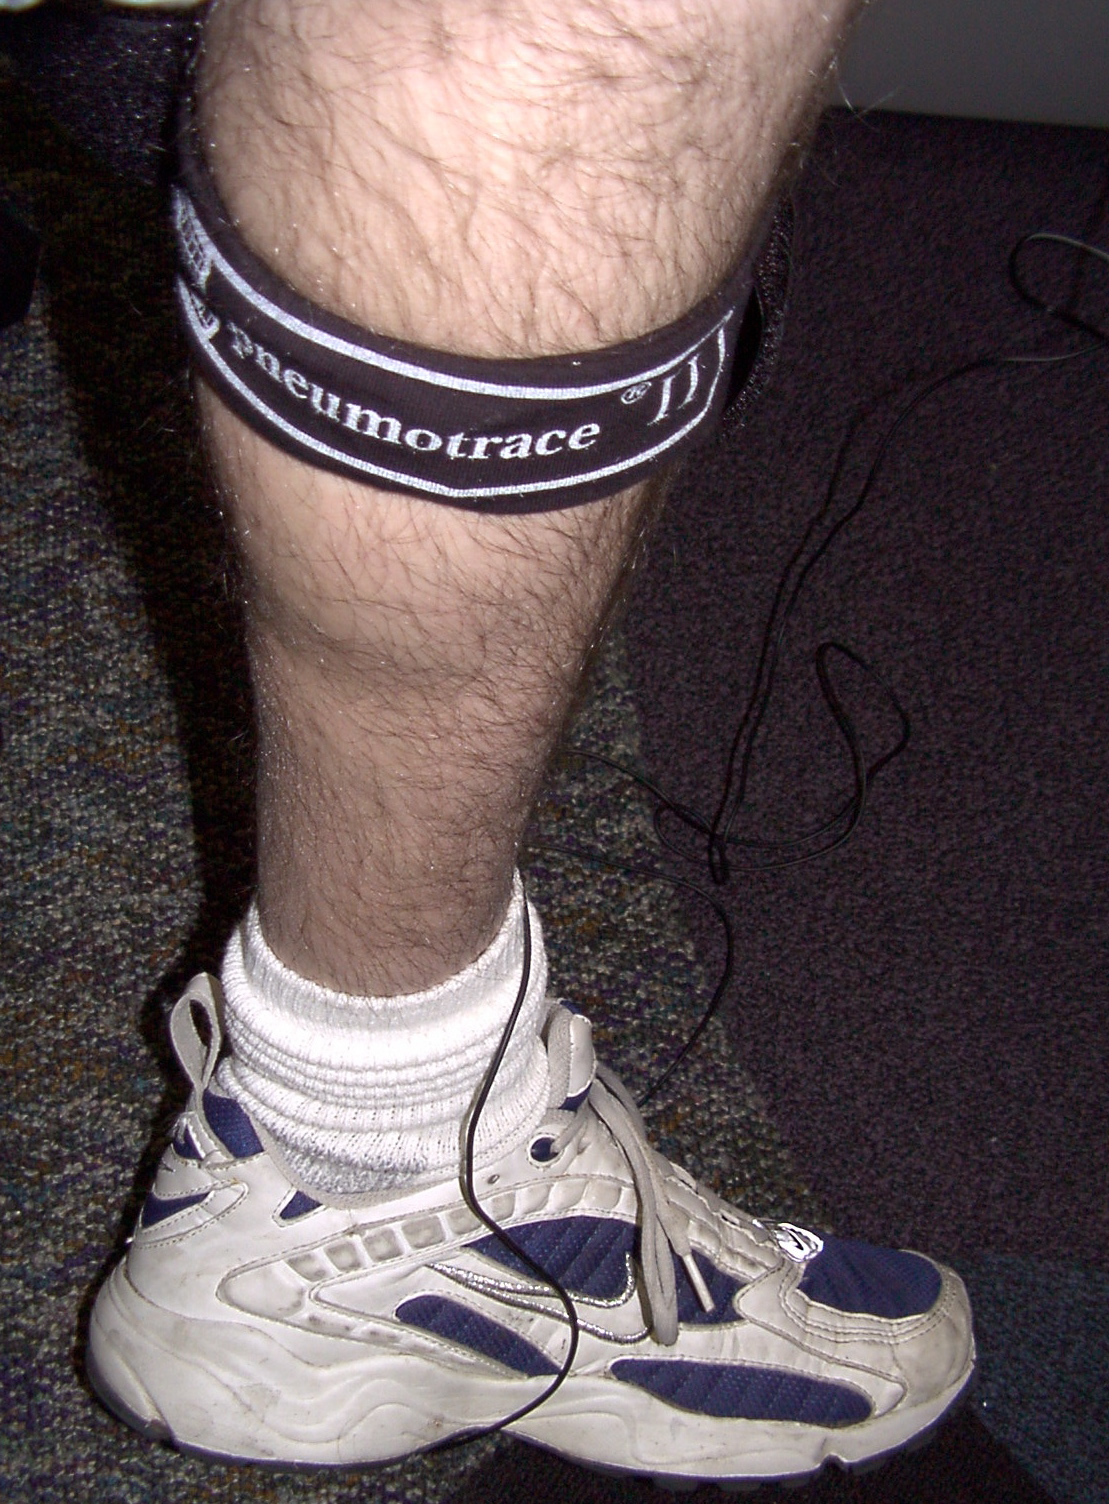
\includegraphics{../../images/calf_belt.jpg}

}

\caption{\label{fig-calf}Attachment of the respiratory belt transducer
to the calf for leg volume measurement.}

\end{marginfigure}

\begin{enumerate}
\def\labelenumi{\arabic{enumi}.}
\tightlist
\item
  Switch the PowerLab to the Dive Response settings. You should have the
  Finger Pulse transducer in channel 1 and the Respiratory Belt
  Transducer to input 2 to measure leg volume. Check the channel
  settings to make sure they match the inputs. Ask your TA for the
  proper settings. In this experiment, the sphygnamanometer is used to
  pressurize the thigh and not plugged in to PowerLab.
\item
  Set up and maintain a wash basin with icewater deep enough to submerge
  your face up to your temples. Use a thermometer to monitor temperature
  at 10-15C (50-60F), replenish with ice as needed.
\item
  Attach the respiratory belt snugly to the calf
  (Figure~\ref{fig-calf}). \emph{It should feel tight and the sensor
  fabric should be slightly stretched.}
\item
  Place the sphygnomanometer cuff around the subject's thigh, and
  \emph{duct tape it securely so that it can be pressurized to restrict
  blood flow}. Be sure to apply tape to \emph{secure both the top and
  the bottom} of the cuff.
\item
  Record for 10 seconds and stop. Scale the Pulse channel and the Leg
  Volume channel to fully display the data.
\item
  Record again and test by flexing and relaxing your calf. \emph{You
  should be able to see a clear deflection on the leg volume channel.}
  If it is very small, try tightening the respiratory belt a little.
  Check with your TA before moving on.
\item
  For all experiments, \emph{resting position for the subject is leaning
  over the basin with the face just aboe water.}
\item
  Use a timer to time the treatments (a cell phone or a web browser will
  do).
\end{enumerate}

\begin{tcolorbox}[enhanced jigsaw, opacityback=0, colbacktitle=quarto-callout-note-color!10!white, opacitybacktitle=0.6, colback=white, leftrule=.75mm, title=\textcolor{quarto-callout-note-color}{\faInfo}\hspace{0.5em}{The idea behind measuring peripheral circulation using leg volume
changes}, breakable, rightrule=.15mm, colframe=quarto-callout-note-color-frame, bottomrule=.15mm, bottomtitle=1mm, arc=.35mm, toptitle=1mm, titlerule=0mm, toprule=.15mm, left=2mm, coltitle=black]

We can quantify the volume in your peripheral circulation (specifically
your lower leg) by assessing \textbf{venous pooling} for a standard time
interval. By constricting blood flow to the lower limb, we will prevent
venous return of the blood. Because the veins have little smooth muscle,
it is relatively easy to stop venous return.

\end{tcolorbox}

\begin{tcolorbox}[enhanced jigsaw, opacityback=0, colbacktitle=quarto-callout-tip-color!10!white, opacitybacktitle=0.6, colback=white, leftrule=.75mm, title=\textcolor{quarto-callout-tip-color}{\faLightbulb}\hspace{0.5em}{Protocol: Basic Leg volume measurement}, breakable, rightrule=.15mm, colframe=quarto-callout-tip-color-frame, bottomrule=.15mm, bottomtitle=1mm, arc=.35mm, toptitle=1mm, titlerule=0mm, toprule=.15mm, left=2mm, coltitle=black]

You will use the sphygnomanometer cuff to cut off circulation in the leg
for 20 sec.~at the upper thigh. The respiratory belt transducer senses
stretch and can be used to measure \textbf{calf volume}
(Figure~\ref{fig-calf}) \textbf{before}, \textbf{during inflation}, and
\textbf{after deflating} the cuff (recovery).

\begin{enumerate}
\def\labelenumi{\arabic{enumi}.}
\tightlist
\item
  Record the subject's \textbf{resting} recording for 10 seconds.
\item
  Rapidly \textbf{Inflate} the cuff to \textbf{60 mmHg} (or whatever
  pressure feels tight enough to restrict blood flow for the subject
  {[}I used 80 mmHg{]}, the pressure should be same for all
  measurements),
\item
  \textbf{Hold pressure} for \textbf{exactly 20 seconds} (\emph{NOTE:
  You may have to gently squeeze the bulb to keep pressure constant.})
\item
  \textbf{Quickly and COMPLETELY release} the pressure
  (Figure~\ref{fig-legvol}).
\item
  \textbf{Recovery:} Record for 30 sec or until the leg volume returns
  to baseline.
\end{enumerate}

\hypertarget{notes-1}{%
\paragraph{NOTES:}\label{notes-1}}

\begin{itemize}
\tightlist
\item
  {Comments should be placed at the \textbf{start of rest} and at the
  \textbf{start} of each change in condition.}
\item
  \emph{Be sure to have the comments pre-typed in the comment box and
  hit enter at the start of each event to accurately place comments in
  time.}
\item
  \textbf{Inflate} and \textbf{deflate} the cuff as fast as possible.
\item
  When doing \emph{repeated measurements}, ensure you have
  \textbf{baseline data} for \emph{at least 15 sec} before inflating the
  cuff again.
\item
  The subject will have to hold their breath for about 30 sec.~
\item
  Make \textbf{good comments} and \textbf{minimize movement} in the
  Finger Pulse Transducer.
\end{itemize}

\end{tcolorbox}

\hypertarget{b.-control-experiment}{%
\subsection{B. Control experiment}\label{b.-control-experiment}}

\begin{enumerate}
\def\labelenumi{\arabic{enumi}.}
\tightlist
\item
  Use the \href{@sec-divesetup}{Section A setup} with the respiratory
  belt on the calf (Figure~\ref{fig-calf}) and the sphygnomanometer cuff
  on the upper thigh.
\item
  Subject leans over basin with face just above water.
\item
  Start recording and comment {``control, resting''}, record for 10sec.
\item
  Rapidly inflate the cuff to 60mmHg, comment {``control, cuff
  inflated''}, and record for 20sec.\\
\item
  Quickly release all cuff pressure, and comment {``deflated''}. Record
  for 30 sec or until leg volume and HR stabilizes.
\end{enumerate}

{Make sure to \textbf{comment at each step} and always \textbf{DEFLATE
CUFF COMPLETELY} each time.}

\hypertarget{c.-dive-response-experiment}{%
\subsection{C. Dive response
experiment}\label{c.-dive-response-experiment}}

\emph{Note: It is critical that the temples be submerged in order to see
the dive response.}

\begin{tcolorbox}[enhanced jigsaw, opacityback=0, colbacktitle=quarto-callout-note-color!10!white, opacitybacktitle=0.6, colback=white, leftrule=.75mm, title=\textcolor{quarto-callout-note-color}{\faInfo}\hspace{0.5em}{NOTES:}, breakable, rightrule=.15mm, colframe=quarto-callout-note-color-frame, bottomrule=.15mm, bottomtitle=1mm, arc=.35mm, toptitle=1mm, titlerule=0mm, toprule=.15mm, left=2mm, coltitle=black]

\begin{itemize}
\tightlist
\item
  \textbf{Make sure everything is very clear before beginning} to avoid
  repeating this experiment.
\item
  It is a good idea to practice a dry run of the simulated dive
  procedure (without submerging face).
\item
  One member of the group should tap the subject on the back at
  10-second intervals while immersed to help them keep track of the time
  and prevent anxiety.
\item
  Work out in advance what your signals will be for timing (10s mark)
  vs.~resurfacing.
\item
  \emph{Do not force the subject to remain submerged}.\\
\end{itemize}

\end{tcolorbox}

\begin{enumerate}
\def\labelenumi{\arabic{enumi}.}
\tightlist
\item
  Use the \href{@sec-divesetup}{Section A setup}. The basin should be in
  front of the subject and at 10-15C.
\item
  Before beginning, allow the subject to find a comforable chair height
  and leg posture to allow them to \emph{remain as motionless as
  possible with their face above the basin}. Most people sit, but
  standing is OK if preferred.
\item
  \textbf{Rest:} Start recording and comment {``dive experiment,
  resting''}, record for 10sec.
\item
  \textbf{Simulated dive:}

  \begin{enumerate}
  \def\labelenumii{\alph{enumii}.}
  \tightlist
  \item
    \textbf{Rapidly} inflate cuff to 60mmHg, comment {``cuff
    inflated''}.\\
  \item
    Have the subject take a deep breath, exhale partially, and then hold
    their breath while immersing their face up to their temples in the
    pan of water. Comment {``dive''}, record for 20 sec.~
  \item
    \textbf{Rapidly} release all cuff pressure. Comment {``deflated''},
    and record for 10 sec.\\
  \item
    Signal to the subject to \textbf{resurface} and breathe normally
    with face just above water. Comment {``normal breathing''} and
    record for 10 sec.~
  \item
    Allow subject to gently dry face.
  \end{enumerate}
\item
  \textbf{Post-dive:} Perform a leg volume measurement post-dive.

  \begin{enumerate}
  \def\labelenumii{\alph{enumii}.}
  \tightlist
  \item
    Comment {``post-dive''} and record for 10 sec.~
  \item
    Rapidly inflate cuff to 60mmHg, comment {``cuff inflated''} and
    record for 20 sec.~
  \item
    Rapidly release all pressure. Comment {``deflated''}, and record for
    10 sec.~
  \end{enumerate}
\end{enumerate}

\hypertarget{c.-breath-holding-exeriment}{%
\subsection{C. Breath holding
exeriment}\label{c.-breath-holding-exeriment}}

\begin{enumerate}
\def\labelenumi{\arabic{enumi}.}
\tightlist
\item
  This experiment is very similar to the dive response, but without
  facial immersion. The subject will remain motionless with their face
  above the basin.
\item
  Record and comment {``breath hold experiment, resting''}. Record for
  10 sec.~
\item
  \textbf{Breath hold:}

  \begin{enumerate}
  \def\labelenumii{\alph{enumii}.}
  \tightlist
  \item
    Rapidly inflate cuff to 60mmHg, comment {``cuff inflated''}.\\
  \item
    Have the subject take a deep breath, exhale partially, and then hold
    their breath. Comment {``breath hold''}, record for 20 sec.~
  \item
    Rapidly release all pressure. Comment {``deflated''}, and record for
    10 sec.\\
  \item
    Signal to the subject to \textbf{breathe normally} with face just
    above water. Comment {``normal breathing''} and record for 10 sec.~
  \end{enumerate}
\end{enumerate}

\hypertarget{d.-additional-experiment}{%
\subsection{D. Additional Experiment}\label{d.-additional-experiment}}

The simulated dive involves multiple stimuli simultaneously.
\textbf{Brainstorm} how you might \emph{identify the components which
are actually ``triggering'' the dive response by isolating stimuli.} Are
these components all necessary? Are they additive?

Each group should \textbf{design and perform an experiment to isolate
one potential stimulus} responsible for triggering the dive response.
Get your idea approved by your TA. Share your results with the other
groups. \emph{Make sure you explain your methods carefully (including
your logic) in your lab report.}

\hypertarget{analysis-1}{%
\subsection{Analysis}\label{analysis-1}}

\hypertarget{change-in-heart-rate-and-pulse-amplitude}{%
\subsubsection{Change in Heart Rate and Pulse
Amplitude}\label{change-in-heart-rate-and-pulse-amplitude}}

\begin{enumerate}
\def\labelenumi{\arabic{enumi}.}
\tightlist
\item
  First analyze the \textbf{Control Experiment} and \textbf{Dive
  Response} data.
\item
  Open the data in the Chart View and \textbf{Autoscale}, if necessary.
  Change the compression of the data trace so the entire exercise can be
  viewed at once. Identify the \textbf{rest} section of the data and
  change the compression to find a representative cycle. \emph{You can
  change the compression and scale as often as required.}
\item
  Move the \textbf{Waveform Cursor} to a representative cycle on the
  \textbf{pulse} channel during \textbf{rest}. Collect the values for
  \textbf{heart rate} and \textbf{pulse amplitude} at the pulse peak.
\item
  Collect \textbf{heart rate} and \textbf{pulse amplitude} for:

  \begin{enumerate}
  \def\labelenumii{\alph{enumii}.}
  \tightlist
  \item
    rest
  \item
    15 sec into the dive (a representative pulsewave during dive)
  \item
    10 sec after the end of the dive (recovery)
  \item
    Tabulate the data in your notebook (for example see
    Table~\ref{tbl-hrdata})
  \end{enumerate}
\item
  For the remaining experiments \textbf{Post Dive}, \textbf{Breath Hold}
  experiment, and \textbf{Your Experiment}, you only need to collect
  heart rate and pulse amplitude data for the treatment period
  (pre-treatment and post-treatment not necessary;
  Table~\ref{tbl-lvdata})
\end{enumerate}

\hypertarget{tbl-hrdata}{}
\begin{longtable}[]{@{}lllll@{}}
\caption{\label{tbl-hrdata}Heart rate and pulse amplitude should be
recorded at rest, during the treatment, and during the recovery for each
experiment.}\tabularnewline
\toprule\noalign{}
Experiment & Parameter & Rest & Treatment & Recovery \\
\midrule\noalign{}
\endfirsthead
\toprule\noalign{}
Experiment & Parameter & Rest & Treatment & Recovery \\
\midrule\noalign{}
\endhead
\bottomrule\noalign{}
\endlastfoot
Control & heart rate (BPM) & & & \\
& pulse amplitude (mV) & & & \\
Dive & heart rate (BPM) & & & \\
& pulse amplitude (mV) & & & \\
\end{longtable}

\hypertarget{change-in-peripheral-circulation}{%
\subsubsection{Change in Peripheral
Circulation}\label{change-in-peripheral-circulation}}

\begin{marginfigure}

{\centering 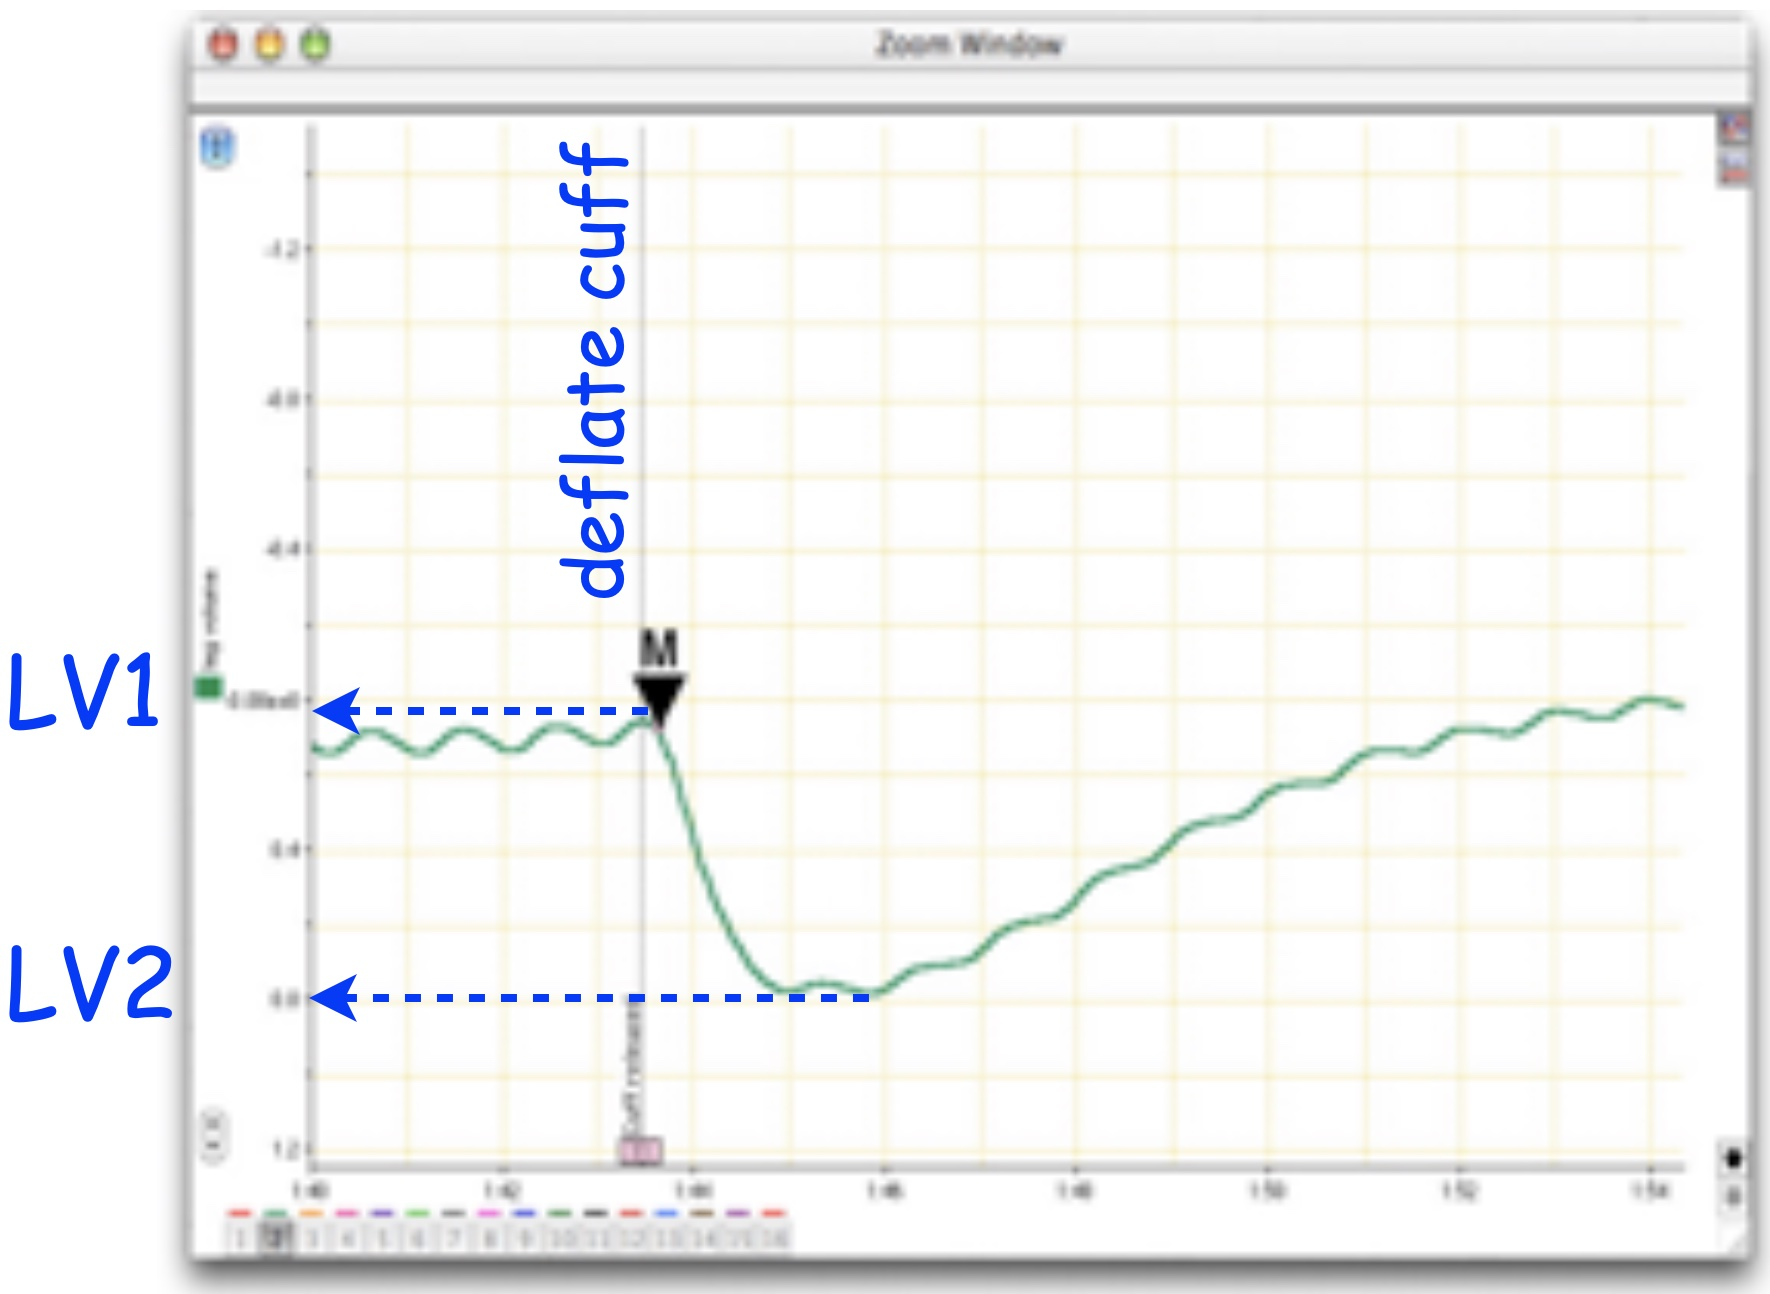
\includegraphics{../../images/legvol.jpg}

}

\caption{\label{fig-legvol}Zoom window view of measuring the leg volume
change resulting from a simulated dive using a marker at T1 (30sec of
cuff inflation) and the waveform cursor at T2 (maximum leg volume drop
after releasing the pressure).}

\end{marginfigure}

\begin{tcolorbox}[enhanced jigsaw, opacityback=0, colbacktitle=quarto-callout-tip-color!10!white, opacitybacktitle=0.6, colback=white, leftrule=.75mm, title=\textcolor{quarto-callout-tip-color}{\faLightbulb}\hspace{0.5em}{Collecting leg volume change from the volume trace:}, breakable, rightrule=.15mm, colframe=quarto-callout-tip-color-frame, bottomrule=.15mm, bottomtitle=1mm, arc=.35mm, toptitle=1mm, titlerule=0mm, toprule=.15mm, left=2mm, coltitle=black]

You will collect the relative signal amplitude change when the cuff
pressure is released.

\begin{enumerate}
\def\labelenumi{\arabic{enumi}.}
\tightlist
\item
  Set the \textbf{Marker} to the point of maximum leg voluime (a region
  just prior to cuff deflation in the leg volume channel;
  Figure~\ref{fig-legvol}).
\item
  Using the \textbf{Waveform Cursor}, obtain the \textbf{difference in
  leg volume} between maximum and minimum leg volume (\(\Delta LV\) (mV)
  \(= LV1 - LV2\); Figure~\ref{fig-legvol}). Note the maximum and
  minimum should be just before and a little after the cuff is deflated.
\item
  \textbf{Relative leg volume} is the ratio between the experimental and
  control leg volume differences.
  \(Rel LV = \Delta LV_{treatment} / \Delta LV_{control}\).
\end{enumerate}

\textbf{The \emph{leg volume} difference} is a measure of pooling and
therefore peripheral circulation. \textbf{Relative leg volume}
quantifies \textbf{changes} in \emph{peripheral circulation}.

\end{tcolorbox}

\begin{enumerate}
\def\labelenumi{\arabic{enumi}.}
\tightlist
\item
  Collect the leg volume difference for the \textbf{control}, during the
  \textbf{dive}, and \textbf{post dive} ( \(\Delta LV_{control}\),
  \(\Delta LV_{dive}\), and \(\Delta LV_{post-dive}\) ) .
\item
  Calculate the relative leg volumes for dive vs.~control and post-dive
  vs.~control ( \(\Delta LV_{dive}/ \Delta LV_{control}\), and
  \(\Delta LV_{post-dive}/ \Delta LV_{control}\) ).
\item
  Do the same for the \textbf{breath hold experiment}, and your
  \textbf{custom experiment} and tabulate as in Table~\ref{tbl-lvdata}.
\end{enumerate}

\hypertarget{tbl-lvdata}{}
\begin{longtable}[]{@{}
  >{\raggedright\arraybackslash}p{(\columnwidth - 10\tabcolsep) * \real{0.1667}}
  >{\raggedright\arraybackslash}p{(\columnwidth - 10\tabcolsep) * \real{0.1667}}
  >{\raggedright\arraybackslash}p{(\columnwidth - 10\tabcolsep) * \real{0.1667}}
  >{\raggedright\arraybackslash}p{(\columnwidth - 10\tabcolsep) * \real{0.1667}}
  >{\raggedright\arraybackslash}p{(\columnwidth - 10\tabcolsep) * \real{0.1667}}
  >{\raggedright\arraybackslash}p{(\columnwidth - 10\tabcolsep) * \real{0.1667}}@{}}
\caption{\label{tbl-lvdata}Heart rate (HR), pulse amplitude (PA), and
leg volume (LV) data to record in your notebook. These are measurements
taken during the ``treatment'' phase of each experiment. You may use the
\(HR_{control}\), \(PA_{control}\), and \(\Delta LV_{control}\) for all
of your comparisions if your setup has not changed (i.e., you did not
reposition your cuff or your transducers).}\tabularnewline
\toprule\noalign{}
\begin{minipage}[b]{\linewidth}\raggedright
\end{minipage} & \begin{minipage}[b]{\linewidth}\raggedright
Control
\end{minipage} & \begin{minipage}[b]{\linewidth}\raggedright
Dive
\end{minipage} & \begin{minipage}[b]{\linewidth}\raggedright
Post Dive
\end{minipage} & \begin{minipage}[b]{\linewidth}\raggedright
Breath Hold
\end{minipage} & \begin{minipage}[b]{\linewidth}\raggedright
My Expt
\end{minipage} \\
\midrule\noalign{}
\endfirsthead
\toprule\noalign{}
\begin{minipage}[b]{\linewidth}\raggedright
\end{minipage} & \begin{minipage}[b]{\linewidth}\raggedright
Control
\end{minipage} & \begin{minipage}[b]{\linewidth}\raggedright
Dive
\end{minipage} & \begin{minipage}[b]{\linewidth}\raggedright
Post Dive
\end{minipage} & \begin{minipage}[b]{\linewidth}\raggedright
Breath Hold
\end{minipage} & \begin{minipage}[b]{\linewidth}\raggedright
My Expt
\end{minipage} \\
\midrule\noalign{}
\endhead
\bottomrule\noalign{}
\endlastfoot
heart rate (BPM) & & & & & \\
pulse amplitude (mv) & & & & & \\
\(\Delta LV\) (mV) & & & & & \\
& & & & & \\
& & \textbf{Dive/Control} & \textbf{Post Dive/Control} & \textbf{Breath
Hold/Control} & \textbf{My Expt/Control} \\
Relative HR & & & & & \\
Relative PA & & & & & \\
Relative LV & & & & & \\
\end{longtable}

\hypertarget{questions-for-thought-.-.-.}{%
\subsection{Questions for thought . .
.}\label{questions-for-thought-.-.-.}}

\begin{enumerate}
\def\labelenumi{\arabic{enumi}.}
\tightlist
\item
  Compare your results of heart rate during breath holding with those
  from simulated dives. Are they the same?
\item
  What factors could explain differences between breath holding and a
  ``dive''? Have you eliminated any hypotheses with your experiments?
\item
  Compare the percent change in heart rate during dives among different
  people. Is the relative or absolute bradycardia similar?\\
\item
  Do your results for leg volume suggest that peripheral circulation
  changes during a dive? during a breath-hold?
\item
  Did your peripheral circulation increase or decrease during a
  ``dive''? during a breath hold?
\item
  What comparisons can you make to dive deeper into your data? Which
  numbers would you look at?
\item
  Why do you think the diving response is considered advantageous?
\end{enumerate}

\hypertarget{after-lab-assignment-week-3}{%
\section{After Lab: Assignment Week
3:}\label{after-lab-assignment-week-3}}

\begin{itemize}
\tightlist
\item
  You will work with your lab group to analyze data, and you may share
  figures if you wish. However, each person will submit an
  \textbf{Individual WorkSheet} {[}\href{Lab3ws.qmd}{html}{]}
\item
  Reminder: \emph{Practical has been moved to next week (week 4) on Lab
  1 material}. Let us know if you want to come in to practice.
\end{itemize}



\end{document}
